% Section: Training data from OpenFAST
\section{Training data from OpenFAST}
\label{sec:data}

\subsection{Runs and partition}
\label{subsec:data_runs}
{\color{revQ1}
The learned models are trained on closed-loop runs of the plant of Section~\ref{sec:reference}, in the configuration qualified there, with the initial blade pitch angle at its equilibrium value of Section~\ref{subsec:aero_verification}. The wind fields were generated as in Section~\ref{subsec:region3_qual}, at the same seven mean wind speeds from 12 to 24~m/s, with five new turbulence seeds that are used neither in the qualification of Section~\ref{subsec:region3_qual} nor in the validation of the reduced-order model of Section~\ref{subsec:rom}. Each run lasted 660~s, and the first 60~s were discarded. Every wind field was simulated twice: once with the reference controller alone (arm X0), and once with an excitation added to its pitch command (arm X3, Section~\ref{subsec:excitation}), so that the pitch angle is not determined by the wind and the rotor speed alone. Table~\ref{tab:E4_matrix} lists the resulting 70 runs and their partition: the first three seeds form the training set, the fourth the validation set and the fifth the test set, the same for every mean wind speed and for both arms, so that no wind realization is shared between two sets.
}

\begin{table}[htbp]
\centering
\caption{{\color{revQ1}Runs of the training dataset: seven mean wind speeds, five turbulence seeds and two arms per seed, X0 (reference controller alone) and X3 (excitation added to its pitch command). The partition is made by seed.}}
\label{tab:E4_matrix}
\begin{tabular}{lccccc}
\toprule
 & \multicolumn{5}{c}{Turbulence seed} \\
\cmidrule(lr){2-6}
Mean wind speed (m/s) & 34001 & 34002 & 34003 & 34004 & 34005 \\
Partition & training & training & training & validation & test \\
\midrule
12 & X0, X3 & X0, X3 & X0, X3 & X0, X3 & X0, X3 \\
14 & X0, X3 & X0, X3 & X0, X3 & X0, X3 & X0, X3 \\
16 & X0, X3 & X0, X3 & X0, X3 & X0, X3 & X0, X3 \\
18 & X0, X3 & X0, X3 & X0, X3 & X0, X3 & X0, X3 \\
20 & X0, X3 & X0, X3 & X0, X3 & X0, X3 & X0, X3 \\
22 & X0, X3 & X0, X3 & X0, X3 & X0, X3 & X0, X3 \\
24 & X0, X3 & X0, X3 & X0, X3 & X0, X3 & X0, X3 \\
\bottomrule
\end{tabular}
\end{table}

\subsection{Pitch excitation}
\label{subsec:excitation}
{\color{revQ1}
The excitation $p(t)$ is a sequence of plateaus at $+1^\circ$ and $-1^\circ$ with alternating signs, each lasting a random time between 0.5 and 3~s after the ramp that leads to it, with ramps at 4~$^\circ$/s, half the maximum pitch rate of the reference controller; it is zero before $t = 60$~s and is drawn with a different random seed in every excited run. Because the reference controller computes its command from the measured pitch angle (Section~\ref{subsec:coupling}), it receives the measured pitch angle minus the value of $p$ applied at the previous time step, and the applied command is its command plus $p$, clipped to $[0^\circ, 30^\circ]$. This entry point of the excitation was retained, among three entry points tried, by an exploratory comparison of eight runs at two mean wind speeds, with a choice rule fixed before the runs. Figure~\ref{fig:E4_excitation} illustrates the excitation and its effect: at 18~m/s, the excited command follows the command of the reference controller with an offset of about one degree, whereas at 12~m/s, where the reference controller often commands the lower bound of $0^\circ$, the negative part of the excitation is clipped, so that the excitation is weaker in the transition range.
}

\begin{figure}[htbp]
\centering
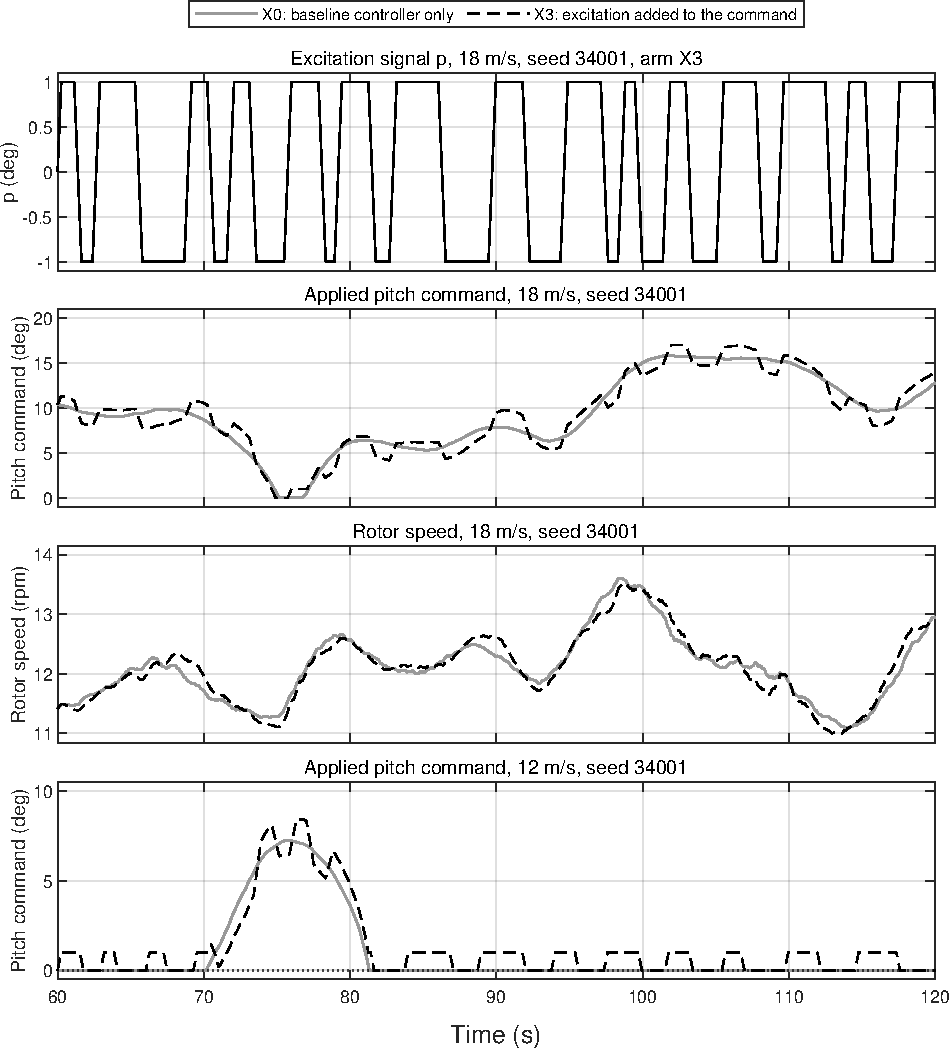
\includegraphics[width=\linewidth]{figures/E4_fig3_excitation.pdf}
\caption{{\color{revQ1}Excitation of the pitch command from 60 to 120~s, seed 34001. From top to bottom: excitation signal $p$ of the excited run at 18~m/s; applied pitch command at 18~m/s with the reference controller alone (X0, grey) and with the excitation (X3, dashed); rotor speed of the same two runs; applied pitch command at 12~m/s, where the dotted line is the lower bound of $0^\circ$ on which the excited command rests when it is clipped.}}
\label{fig:E4_excitation}
\end{figure}

\subsection{Samples and targets}
\label{subsec:samples}
{\color{revQ1}
The dataset is built at the sample time of the NMPC, $T_s = 0.05$~s, from the outputs recorded every 0.00625~s. Its state is $x = [\omega_r, \omega_f]$ and its input is the applied collective pitch command (Section~\ref{subsec:rom}); its disturbance is the rotor-effective wind speed, assumed known as in Section~\ref{subsec:rom}, and the wind speed at hub height is kept in the dataset but is not an input. Figure~\ref{fig:E4_sampling} illustrates the construction of the samples: the state is sampled every $T_s$ from $t = 60$~s, the input and the disturbance are taken at the start of each step and held over it, and the learning target is the state increment $\Delta x_k = x_{k+1} - x_k$, computed only between two consecutive samples of the same run. The mean and the standard deviation used to normalize every variable, the targets included, are computed on the training set only, both arms together. Datasets at 0.025~s and 0.1~s are built from the same runs by the same rule for the sensitivity study. Every run met the execution and pitch-loop criteria of Section~\ref{subsec:region3_qual}, and the dataset was declared ready by a rule fixed before the runs.
}

\begin{figure}[htbp]
\centering
% Figure E4-2 of Paper_Q1 (section 4): sampling of the dataset. Schematic only: no data and no result
% number; the heights of the held values are arbitrary (openfast_q1/docs/spec_figures_E3_E4.yaml,
% E4_2_sampling and general.schematics).
% Content (spec_E4 signals.sampling, signals.target): output grid at DT = 0.00625 s; samples at
% Ts = 0.05 s, one every 8 output steps, from t = 60 s; x_k sampled, u_k and d_k taken at the start of
% the step and held over it; Delta x_k = x_{k+1} - x_k between two samples of the same run; the 60 s
% boundary and the absence of a difference across two runs are marked.
% Requires \usepackage{tikz}, \usetikzlibrary{arrows.meta, positioning, calc} and siunitx
% (Paper_Q1/main.tex). Included with % Figure E4-2 of Paper_Q1 (section 4): sampling of the dataset. Schematic only: no data and no result
% number; the heights of the held values are arbitrary (openfast_q1/docs/spec_figures_E3_E4.yaml,
% E4_2_sampling and general.schematics).
% Content (spec_E4 signals.sampling, signals.target): output grid at DT = 0.00625 s; samples at
% Ts = 0.05 s, one every 8 output steps, from t = 60 s; x_k sampled, u_k and d_k taken at the start of
% the step and held over it; Delta x_k = x_{k+1} - x_k between two samples of the same run; the 60 s
% boundary and the absence of a difference across two runs are marked.
% Requires \usepackage{tikz}, \usetikzlibrary{arrows.meta, positioning, calc} and siunitx
% (Paper_Q1/main.tex). Included with % Figure E4-2 of Paper_Q1 (section 4): sampling of the dataset. Schematic only: no data and no result
% number; the heights of the held values are arbitrary (openfast_q1/docs/spec_figures_E3_E4.yaml,
% E4_2_sampling and general.schematics).
% Content (spec_E4 signals.sampling, signals.target): output grid at DT = 0.00625 s; samples at
% Ts = 0.05 s, one every 8 output steps, from t = 60 s; x_k sampled, u_k and d_k taken at the start of
% the step and held over it; Delta x_k = x_{k+1} - x_k between two samples of the same run; the 60 s
% boundary and the absence of a difference across two runs are marked.
% Requires \usepackage{tikz}, \usetikzlibrary{arrows.meta, positioning, calc} and siunitx
% (Paper_Q1/main.tex). Included with \input{figures/E4_fig2_sampling} inside a figure environment of
% section 4 (step 5 of spec_figures_E3_E4 order).
\begin{tikzpicture}[
    >={Stealth[length=2mm]},
    lab/.style={font=\footnotesize, align=center}
  ]
  \pgfmathsetmacro{\sTs}{3.0}     % drawing length of one Ts (cm)
  \pgfmathsetmacro{\sDT}{0.375}   % drawing length of one DT (cm), Ts / 8
  % ---------------- one run around t = 60 s ----------------
  \fill[gray!15] (-1.5, -0.1) rectangle (0, 2.9);
  \node[lab] at (-0.75, 2.5) {excluded\\$t < \SI{60}{\second}$};
  \draw[->] (-1.5, 0) -- (9.9, 0) node[lab, right] {$t$};
  \foreach \i in {-4,...,25} \draw (\sDT*\i, 0) -- ++(0, 0.1);            % output grid (DT)
  \foreach \k in {0, 1, 2, 3} \draw[thick] (\sTs*\k, -0.15) -- (\sTs*\k, 0.2);   % samples (Ts)
  \node[lab, below] at (0, -0.15) {$t_0 = \SI{60}{\second}$};
  \foreach \k in {1, 2, 3} \node[lab, below] at (\sTs*\k, -0.15) {$t_{\k}$};
  \draw[dashed] (0, -0.1) -- (0, 2.9);                                       % 60 s boundary
  % sampling period and output step
  \draw[<->] (0, -0.95) -- node[lab, below] {$T_s = \SI{0.05}{\second} = 8\,\mathrm{DT}$} (\sTs, -0.95);
  \draw[<->] (2*\sTs, -0.95) -- (2*\sTs + \sDT, -0.95)
    node[lab, right] {$\mathrm{DT} = 0.00625\,\mathrm{s}$ (output grid)};
  % input and disturbance: value at the start of the step, held over it
  \foreach \k/\y in {0/0.6, 1/0.95, 2/0.75} {
    \draw[thick] (\sTs*\k, \y) -- (\sTs*\k + \sTs, \y);
    \fill (\sTs*\k, \y) circle (1.5pt);
    \draw[fill=white] (\sTs*\k + \sTs, \y) circle (1.5pt);
    \node[lab, above] at (\sTs*\k + 0.5*\sTs, \y) {$u_{\k}, d_{\k}$};
  }
  % sampled state and target
  \foreach \k in {0, 1, 2, 3} {
    \fill (\sTs*\k, 2.0) circle (2pt);
    \node[lab, below right] at (\sTs*\k, 2.0) {$x_{\k}$};
  }
  \foreach \k in {0, 1, 2}
    \draw[->] (\sTs*\k + 0.1, 2.1) to[bend left=30] node[lab, above] {$\Delta x_{\k}$} (\sTs*\k + \sTs - 0.1, 2.1);
  % reading of the row
  \node[lab, align=left, anchor=west] at (10.4, 2.0) {$x_k$ sampled at $t_k$\\$\Delta x_k = x_{k+1} - x_k$};
  \node[lab, align=left, anchor=west] at (10.4, 0.8) {$u_k$, $d_k$: value at $t_k$,\\held over $[t_k, t_{k+1})$};
  % ---------------- no difference across two runs ----------------
  \begin{scope}[yshift=-3.9cm]
    \draw (-1.5, 0) -- (4.2, 0);
    \node[lab, anchor=west] at (-1.5, 2.2) {run $r$ (end)};
    \foreach \x in {0.6, 3.6} {
      \draw[thick] (\x, -0.15) -- (\x, 0.2);
      \fill (\x, 0.9) circle (2pt);
    }
    \node[lab, below] at (0.6, -0.15) {$t_{K-1}$};
    \node[lab, below] at (3.6, -0.15) {$t_K$};
    \node[lab, below right] at (0.6, 0.9) {$x_{K-1}$};
    \node[lab, below right] at (3.6, 0.9) {$x_K$};
    \draw[->] (0.7, 1.0) to[bend left=30] node[lab, above] {$\Delta x_{K-1}$} (3.5, 1.0);
    \draw[->] (6.0, 0) -- (9.9, 0) node[lab, right] {$t$};
    \node[lab, anchor=west] at (6.0, 2.2) {run $r+1$ (start)};
    \draw[thick] (6.6, -0.15) -- (6.6, 0.2);
    \node[lab, below] at (6.6, -0.15) {$t_0 = \SI{60}{\second}$};
    \fill (6.6, 0.9) circle (2pt);
    \node[lab, below right] at (6.6, 0.9) {$x_0$};
    \draw[->, dashed] (3.75, 0.9) -- (6.45, 0.9);
    \draw[thick] (5.1, 0.9) +(-0.15, -0.15) -- +(0.15, 0.15) +(-0.15, 0.15) -- +(0.15, -0.15);
    \node[lab, above] at (5.1, 1.05) {no $\Delta x$ across\\two runs};
  \end{scope}
\end{tikzpicture}
 inside a figure environment of
% section 4 (step 5 of spec_figures_E3_E4 order).
\begin{tikzpicture}[
    >={Stealth[length=2mm]},
    lab/.style={font=\footnotesize, align=center}
  ]
  \pgfmathsetmacro{\sTs}{3.0}     % drawing length of one Ts (cm)
  \pgfmathsetmacro{\sDT}{0.375}   % drawing length of one DT (cm), Ts / 8
  % ---------------- one run around t = 60 s ----------------
  \fill[gray!15] (-1.5, -0.1) rectangle (0, 2.9);
  \node[lab] at (-0.75, 2.5) {excluded\\$t < \SI{60}{\second}$};
  \draw[->] (-1.5, 0) -- (9.9, 0) node[lab, right] {$t$};
  \foreach \i in {-4,...,25} \draw (\sDT*\i, 0) -- ++(0, 0.1);            % output grid (DT)
  \foreach \k in {0, 1, 2, 3} \draw[thick] (\sTs*\k, -0.15) -- (\sTs*\k, 0.2);   % samples (Ts)
  \node[lab, below] at (0, -0.15) {$t_0 = \SI{60}{\second}$};
  \foreach \k in {1, 2, 3} \node[lab, below] at (\sTs*\k, -0.15) {$t_{\k}$};
  \draw[dashed] (0, -0.1) -- (0, 2.9);                                       % 60 s boundary
  % sampling period and output step
  \draw[<->] (0, -0.95) -- node[lab, below] {$T_s = \SI{0.05}{\second} = 8\,\mathrm{DT}$} (\sTs, -0.95);
  \draw[<->] (2*\sTs, -0.95) -- (2*\sTs + \sDT, -0.95)
    node[lab, right] {$\mathrm{DT} = 0.00625\,\mathrm{s}$ (output grid)};
  % input and disturbance: value at the start of the step, held over it
  \foreach \k/\y in {0/0.6, 1/0.95, 2/0.75} {
    \draw[thick] (\sTs*\k, \y) -- (\sTs*\k + \sTs, \y);
    \fill (\sTs*\k, \y) circle (1.5pt);
    \draw[fill=white] (\sTs*\k + \sTs, \y) circle (1.5pt);
    \node[lab, above] at (\sTs*\k + 0.5*\sTs, \y) {$u_{\k}, d_{\k}$};
  }
  % sampled state and target
  \foreach \k in {0, 1, 2, 3} {
    \fill (\sTs*\k, 2.0) circle (2pt);
    \node[lab, below right] at (\sTs*\k, 2.0) {$x_{\k}$};
  }
  \foreach \k in {0, 1, 2}
    \draw[->] (\sTs*\k + 0.1, 2.1) to[bend left=30] node[lab, above] {$\Delta x_{\k}$} (\sTs*\k + \sTs - 0.1, 2.1);
  % reading of the row
  \node[lab, align=left, anchor=west] at (10.4, 2.0) {$x_k$ sampled at $t_k$\\$\Delta x_k = x_{k+1} - x_k$};
  \node[lab, align=left, anchor=west] at (10.4, 0.8) {$u_k$, $d_k$: value at $t_k$,\\held over $[t_k, t_{k+1})$};
  % ---------------- no difference across two runs ----------------
  \begin{scope}[yshift=-3.9cm]
    \draw (-1.5, 0) -- (4.2, 0);
    \node[lab, anchor=west] at (-1.5, 2.2) {run $r$ (end)};
    \foreach \x in {0.6, 3.6} {
      \draw[thick] (\x, -0.15) -- (\x, 0.2);
      \fill (\x, 0.9) circle (2pt);
    }
    \node[lab, below] at (0.6, -0.15) {$t_{K-1}$};
    \node[lab, below] at (3.6, -0.15) {$t_K$};
    \node[lab, below right] at (0.6, 0.9) {$x_{K-1}$};
    \node[lab, below right] at (3.6, 0.9) {$x_K$};
    \draw[->] (0.7, 1.0) to[bend left=30] node[lab, above] {$\Delta x_{K-1}$} (3.5, 1.0);
    \draw[->] (6.0, 0) -- (9.9, 0) node[lab, right] {$t$};
    \node[lab, anchor=west] at (6.0, 2.2) {run $r+1$ (start)};
    \draw[thick] (6.6, -0.15) -- (6.6, 0.2);
    \node[lab, below] at (6.6, -0.15) {$t_0 = \SI{60}{\second}$};
    \fill (6.6, 0.9) circle (2pt);
    \node[lab, below right] at (6.6, 0.9) {$x_0$};
    \draw[->, dashed] (3.75, 0.9) -- (6.45, 0.9);
    \draw[thick] (5.1, 0.9) +(-0.15, -0.15) -- +(0.15, 0.15) +(-0.15, 0.15) -- +(0.15, -0.15);
    \node[lab, above] at (5.1, 1.05) {no $\Delta x$ across\\two runs};
  \end{scope}
\end{tikzpicture}
 inside a figure environment of
% section 4 (step 5 of spec_figures_E3_E4 order).
\begin{tikzpicture}[
    >={Stealth[length=2mm]},
    lab/.style={font=\footnotesize, align=center}
  ]
  \pgfmathsetmacro{\sTs}{3.0}     % drawing length of one Ts (cm)
  \pgfmathsetmacro{\sDT}{0.375}   % drawing length of one DT (cm), Ts / 8
  % ---------------- one run around t = 60 s ----------------
  \fill[gray!15] (-1.5, -0.1) rectangle (0, 2.9);
  \node[lab] at (-0.75, 2.5) {excluded\\$t < \SI{60}{\second}$};
  \draw[->] (-1.5, 0) -- (9.9, 0) node[lab, right] {$t$};
  \foreach \i in {-4,...,25} \draw (\sDT*\i, 0) -- ++(0, 0.1);            % output grid (DT)
  \foreach \k in {0, 1, 2, 3} \draw[thick] (\sTs*\k, -0.15) -- (\sTs*\k, 0.2);   % samples (Ts)
  \node[lab, below] at (0, -0.15) {$t_0 = \SI{60}{\second}$};
  \foreach \k in {1, 2, 3} \node[lab, below] at (\sTs*\k, -0.15) {$t_{\k}$};
  \draw[dashed] (0, -0.1) -- (0, 2.9);                                       % 60 s boundary
  % sampling period and output step
  \draw[<->] (0, -0.95) -- node[lab, below] {$T_s = \SI{0.05}{\second} = 8\,\mathrm{DT}$} (\sTs, -0.95);
  \draw[<->] (2*\sTs, -0.95) -- (2*\sTs + \sDT, -0.95)
    node[lab, right] {$\mathrm{DT} = 0.00625\,\mathrm{s}$ (output grid)};
  % input and disturbance: value at the start of the step, held over it
  \foreach \k/\y in {0/0.6, 1/0.95, 2/0.75} {
    \draw[thick] (\sTs*\k, \y) -- (\sTs*\k + \sTs, \y);
    \fill (\sTs*\k, \y) circle (1.5pt);
    \draw[fill=white] (\sTs*\k + \sTs, \y) circle (1.5pt);
    \node[lab, above] at (\sTs*\k + 0.5*\sTs, \y) {$u_{\k}, d_{\k}$};
  }
  % sampled state and target
  \foreach \k in {0, 1, 2, 3} {
    \fill (\sTs*\k, 2.0) circle (2pt);
    \node[lab, below right] at (\sTs*\k, 2.0) {$x_{\k}$};
  }
  \foreach \k in {0, 1, 2}
    \draw[->] (\sTs*\k + 0.1, 2.1) to[bend left=30] node[lab, above] {$\Delta x_{\k}$} (\sTs*\k + \sTs - 0.1, 2.1);
  % reading of the row
  \node[lab, align=left, anchor=west] at (10.4, 2.0) {$x_k$ sampled at $t_k$\\$\Delta x_k = x_{k+1} - x_k$};
  \node[lab, align=left, anchor=west] at (10.4, 0.8) {$u_k$, $d_k$: value at $t_k$,\\held over $[t_k, t_{k+1})$};
  % ---------------- no difference across two runs ----------------
  \begin{scope}[yshift=-3.9cm]
    \draw (-1.5, 0) -- (4.2, 0);
    \node[lab, anchor=west] at (-1.5, 2.2) {run $r$ (end)};
    \foreach \x in {0.6, 3.6} {
      \draw[thick] (\x, -0.15) -- (\x, 0.2);
      \fill (\x, 0.9) circle (2pt);
    }
    \node[lab, below] at (0.6, -0.15) {$t_{K-1}$};
    \node[lab, below] at (3.6, -0.15) {$t_K$};
    \node[lab, below right] at (0.6, 0.9) {$x_{K-1}$};
    \node[lab, below right] at (3.6, 0.9) {$x_K$};
    \draw[->] (0.7, 1.0) to[bend left=30] node[lab, above] {$\Delta x_{K-1}$} (3.5, 1.0);
    \draw[->] (6.0, 0) -- (9.9, 0) node[lab, right] {$t$};
    \node[lab, anchor=west] at (6.0, 2.2) {run $r+1$ (start)};
    \draw[thick] (6.6, -0.15) -- (6.6, 0.2);
    \node[lab, below] at (6.6, -0.15) {$t_0 = \SI{60}{\second}$};
    \fill (6.6, 0.9) circle (2pt);
    \node[lab, below right] at (6.6, 0.9) {$x_0$};
    \draw[->, dashed] (3.75, 0.9) -- (6.45, 0.9);
    \draw[thick] (5.1, 0.9) +(-0.15, -0.15) -- +(0.15, 0.15) +(-0.15, 0.15) -- +(0.15, -0.15);
    \node[lab, above] at (5.1, 1.05) {no $\Delta x$ across\\two runs};
  \end{scope}
\end{tikzpicture}

\caption{{\color{revQ1}Construction of the samples at the NMPC sample time $T_s = 8\,\mathrm{DT}$ from the output grid $\mathrm{DT} = 0.00625$~s. Top: one run around $t = 60$~s; the input $u_k$ and the disturbance $d_k$ are held over $[t_k, t_{k+1})$, and the target is $\Delta x_k$. Bottom: no increment is computed across two runs.}}
\label{fig:E4_sampling}
\end{figure}
